\documentclass[10pt,times]{beamer}
\input{preamble.tex}
\subtitle{\LaTeX, vector graphics, reference management and version control}
%***************************** Title page **************************************
\begin{document}
\begin{frame}
  \titlepage
\end{frame}

%*******************************************************************************
%******************************* Frame *****************************************
%*******************************************************************************
\section{World outside the WYSIWYG bubble}

\begin{frame}{Why you shouldn't use Word to write your thesis}
  \centering
  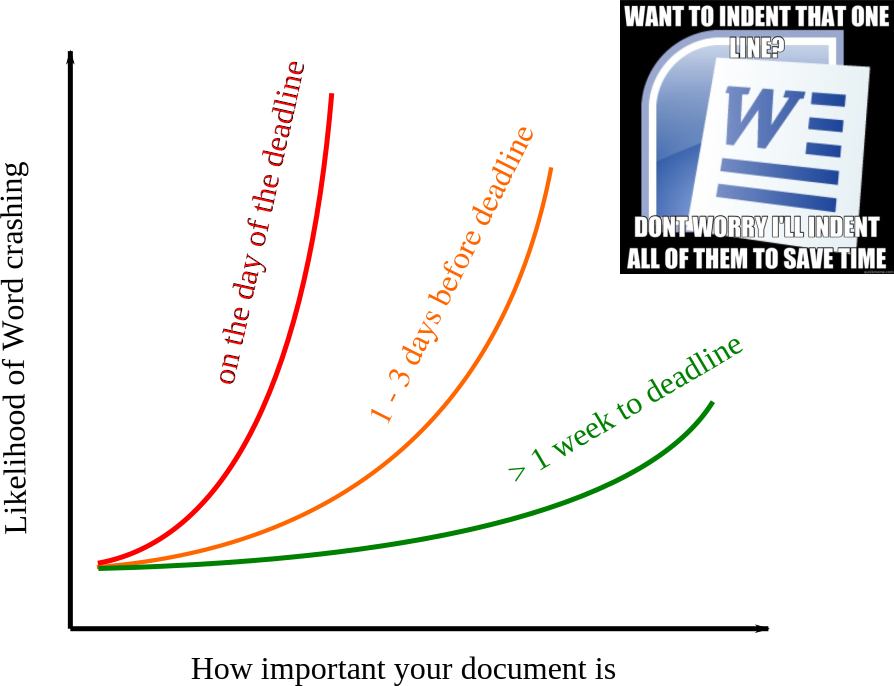
\includegraphics[height=0.8\textheight]{figs/word_crash}
\end{frame}

%*******************************************************************************
%******************************* Frame *****************************************
%*******************************************************************************
\begin{frame}{Can you see beyond the WYSIWYG bubble?}
  \begin{figure}
    \centering
    \includegraphics[height=0.8\textheight]{figs/LaTeX_Word.pdf}
    \caption*{Word vs. \LaTeX}
\end{figure}
\end{frame}

%*******************************************************************************
%******************************* Frame *****************************************
%*******************************************************************************
\begin{frame}{Can you see beyond the WYSIWYG bubble?}
  \begin{figure}
    \centering
    \includegraphics[width=\linewidth]{figs/LaTeX_InDesign_Word.png}
    \caption*{Word vs. InDesign vs. \LaTeX}
\end{figure}
\end{frame}

%*******************************************************************************
%******************************* Frame *****************************************
%*******************************************************************************
\begin{frame}{Ligatures, smallcaps, kerning}
\begin{figure}
  \centering
  \includegraphics[width=0.7\textwidth]{figs/ligatures.png}
  \caption*{Ligatures}
\end{figure}
\begin{figure}
  \centering
  \includegraphics[width=0.4\textwidth]{figs/smallcaps.png}
  \caption*{Smallcaps}
\end{figure}
\begin{figure}
  \centering
  \includegraphics[width=0.4\textwidth]{figs/kerning.png}
  \caption*{Kerning}
\end{figure}
\end{frame}


\section{Introduction to \LaTeX2e}

%*******************************************************************************
%******************************* Frame *****************************************
%*******************************************************************************
\subsection{What is \LaTeX}
\begin{frame}{What is \LaTeX?}
\begin{itemize}
\item \LaTeX is a document preparation system for the \TeX typesetting 
program. 

\item Programmable desktop publishing, which automates most of the typesetting.

\item \LaTeX produce beautiful documents, especially mathematics
\begin{equation*}
i \hbar \frac{\partial}{\partial t} \Psi(r,t) = 
\left[\frac{-\hbar^2}{2\mu}\nabla^2+V(r,t)\right]\Psi(r,t)
\end{equation*}

\begin{equation*}
E^2 = (pc)^2 + (m_0 c^2)^2
\end{equation*}

\item \LaTeX is WYSIWYM (What You See is What You Mean)

\end{itemize}
\end{frame}


%*******************************************************************************
%******************************* Frame *****************************************
%*******************************************************************************
\begin{frame}
\frametitle{History}
It all started with Donald Knuth and ``The Art of Computer Programming'' 
\begin{itemize}
\item
\parbox{0.25\textwidth}{
	\includegraphics[width=0.15\textwidth]{figs/Donald_Knuth.png}}
\parbox{0.65\textwidth}{Donald Knuth, 1977, \TeX - a computer language used for 
typesetting math and other technical material}

\item
\parbox{0.25\textwidth}{\includegraphics[width=0.15\textwidth]{figs/Leslie.png}}
\parbox{0.65\textwidth}{Leslie Lamport, \LaTeX - a higher-level method of 
accessing the power of \TeX}
\end{itemize}
\end{frame}


%*******************************************************************************
%******************************* Frame *****************************************
%*******************************************************************************

\begin{frame}{\LaTeX Pros and Cons}
\textbf{Pros}
\begin{itemize}
\item    It's free and works on Macs, Windows, Unix/Linux.
\item    LaTeX files are ASCII and are portable.
\item    The typesetting is better, especially the maths.
\item    Style changes are neater in LaTeX.
\end{itemize}
\textbf{Cons}
\begin{itemize}
\item    Special/Modern Font selection is difficult, but one can use XeTeX.
\item    LaTeX encourages (almost insists on) structured writing and the 
separation of style from content. This is not the way that many people 
(especially non-programmers) are used to working.
\item    Without a WYSIWYG front end, it's not always easy to find out how to 
do things.
\end{itemize}
\end{frame}

%*******************************************************************************
%******************************* Frame *****************************************
%*******************************************************************************
\subsection{Getting started with \LaTeX}
\begin{frame}{Getting started with \LaTeX}
\begin{itemize}
\item \textbf{Typesetting}
\begin{itemize}
\item \TeX Live - full version
\item MiK\TeX - Windows (Basic installer)
\end{itemize}
\item \textbf{Off-line editors}
\begin{itemize}
\item \TeX Studio
\item \TeX MakerX
\end{itemize}
\item \textbf{Online editors \& \LaTeX compilers}
\begin{itemize}
\item Overleaf (formerly Write\LaTeX)
\item Share\LaTeX
\end{itemize}

\end{itemize}

\end{frame}

%*******************************************************************************
%******************************* Frame *****************************************
%*******************************************************************************
\begin{frame}{How \LaTeX works? - The Magic}
\begin{itemize}
\item You write your document in \texttt{plain text} with \cmmd{commands} that
describe its structure and meaning.
\item The \LaTeX program processes your text and commands to produce a
beautifully formatted document.
\end{itemize}

\centering
\includegraphics[width=0.95\textwidth]{figs/magic.png}
\end{frame}

%*******************************************************************************
%******************************* Frame *****************************************
%*******************************************************************************
\begin{frame}[fragile]{More examples of commands and their output\ldots}
\begin{exampletwoup}
\begin{itemize}
\item Despicable Me
\item Wall-E
\item Tangled
\end{itemize}
\end{exampletwoup}
\vskip 2ex
\begin{exampletwoup}
\begin{figure}
\includegraphics{figs/minion}
\end{figure}
\end{exampletwoup}
\vskip 2ex
\begin{exampletwoup}
\begin{equation}
\alpha = \beta + 1
\end{equation}
\end{exampletwoup}
\end{frame}

%*******************************************************************************
%******************************* Frame *****************************************
%*******************************************************************************
\begin{frame}[fragile]{Getting Started}
\begin{itemize}
\item A minimal \LaTeX{} document:
\inputminted[frame=single]{latex}{Hello.tex}
\item Commands start with a \emph{backslash} \keys{$\backslash$}
\item Every document starts with a \cmdbs{documentclass} command.
\item The \emph{argument} in curly braces \keys{\{} \keys{\}} 
tells \LaTeX what kind of document we are creating: an \bftt{article}.
\item A percent sign \keys{\%} starts a \emph{comment} --- \LaTeX
will ignore the rest of the line.

\end{itemize}
\end{frame}

%*******************************************************************************
%******************************* Frame *****************************************
%*******************************************************************************
\begin{frame}{Declarations and Environments}
\begin{block}{Declaration and commands\ldots}
\begin{itemize}
\item Are stated once
\item Take effect until further notice
\item Can optionally be constrained
\end{itemize}
Eg., \cmdbs{documentclass} or \cmdbs{includegraphics}
\end{block}

\begin{block}{Environments\ldots}
\begin{itemize}
\item Have matching begin and end declarations
\item Must be constrained
\end{itemize}
Eg., \cmdbegin{document} \ldots \cmdend{document}
\end{block}
\end{frame}


%*******************************************************************************
%******************************* Frame *****************************************
%*******************************************************************************
\begin{frame}{Arguments}
\begin{block}{Required arguments\ldots}
\begin{itemize}
\item Are contained in curly braces
\item Must be provided
\end{itemize}
Eg., \cmdbs{documentclass\{article\}}
\end{block}

\begin{block}{Optional arguments\ldots}
\begin{itemize}
\item Are contained in square bracket
\item Can be left out, in which case default value is assumed
\item Give you more control over the commands
\end{itemize}
Eg., \cmdbs{documentclass\lbrack12pt\rbrack\{article\}}
\end{block}
\end{frame}


%*******************************************************************************
%******************************* Frame *****************************************
%*******************************************************************************

\begin{frame}[fragile]{Title and Author}
\begin{itemize}{\small
\item Tell \LaTeX{} the \cmdbs{title} and \cmdbs{author} names in the preamble.
\item Then use \cmdbs{maketitle} in the document to actually create the title.
\item Use the \bftt{abstract} environment to make an abstract.
}\end{itemize}
\centering
\begin{minipage}{0.45\linewidth}
\inputminted[fontsize=\scriptsize,frame=single,resetmargins]{latex}%
  {structure-title.tex}
\end{minipage}
\begin{minipage}{0.45\linewidth}
\includegraphics[width=\textwidth,clip,trim=2.2in 7in 2.2in 
2in]{structure-title.pdf}
\end{minipage}
\end{frame}



%*******************************************************************************
%******************************* Frame *****************************************
%*******************************************************************************
\begin{frame}{Sections}
\begin{minipage}{0.55\linewidth}
\inputminted[fontsize=\scriptsize,frame=single,resetmargins]{latex}%
  {structure-sections.tex}
\end{minipage}
\begin{minipage}{0.35\linewidth}
\includegraphics[width=\textwidth,clip,trim=1.5in 6in 4in 
1in]{structure-sections.pdf}
\end{minipage}
\end{frame}

%*******************************************************************************
%******************************* Frame *****************************************
%*******************************************************************************
\subsection{Example}
\begin{frame}{Let's try that \dots}
\begin{itemize}
\item write\LaTeX{} is a website for writing documents in \LaTeX.
\item It `compiles' your \LaTeX{} automatically to show you the results.
\vskip 2em
\begin{center}
\fbox{\href{\wlnewdoc{paper.tex}}{%
Click here to open the example document in \wllogo{}}}
\\[1ex]\scriptsize{}Or go to this URL: 
\url{\wlserver/docs/1778557gcvcyt/clone}\\
For best results, please use \href{http://www.google.com/chrome}{Google Chrome} 
or a recent \href{http://www.mozilla.org/en-US/firefox/new/}{FireFox}.
\end{center}
\item If you would like to try out the exercise on your machine. Go to 
\cmmd{Exercise / paper.tex}
\end{itemize}
\end{frame}

%*******************************************************************************
%******************************* Frame *****************************************
%*******************************************************************************
\section{How \LaTeX works}

%*******************************************************************************
%******************************* Frame *****************************************
%*******************************************************************************
\begin{frame}{\bs documentclass\{\}}

\begin{table}
\renewcommand{\arraystretch}{1.5}
\begin{tabularx}{0.9\textwidth}{l X}
\toprule
minimal & Is as small as it can get. For debugging purposes.\\ 
letter & For writing letters. \\ 
article & articles in journals, documentation, invitations, \dots \\ 
proc & A class for proceedings based on the article class.\\ 
report & For longer reports containing several chapters \dots \\
book & For real books.\\
memoir & For advanced book style. \\
beamer& For writing presentations \\ \bottomrule
\end{tabularx}
\end{table}
\end{frame}

%*******************************************************************************
%******************************* Frame *****************************************
%*******************************************************************************
\begin{frame}{LaTeX Structure - The Magic}
\begin{figure}
\centering
\includegraphics[height=0.95\textheight]{figs/LaTeX.png}
\end{figure}
\end{frame}

%*******************************************************************************
%******************************* Frame *****************************************
%*******************************************************************************
\begin{frame}{LaTeX - Tool chains}
\begin{figure}
\centering
\includegraphics[width=0.85\textwidth]{figs/Latex-file-flow.png}
\end{figure}
\end{frame}

%*******************************************************************************
%******************************* Frame *****************************************
%*******************************************************************************
\begin{frame}{Packages}
Packages allow you to further customize \LaTeX
\begin{block}{The command:}
\cmdbs{usepackage\{amsmath\}}
\end{block}

\begin{block}{Common packages}
\begin{tabularx}{0.95\textwidth}{lX}
\toprule
Environment & Packages \\ \midrule
Maths & amsmath, amsfonts, amssymb \\ 
Maths Times Font & {mathptx} \\
Figures & graphicx, epsfig \\
Table & tabularx, booktabs \\
Pagelayout & geometry \\
Hyperlinks & hyperref \\
Algorithms and code & algpseudocode, algorithm, listings \\
Color & color, xcolor \\
\bottomrule
\end{tabularx}
\end{block}
\end{frame}


%*******************************************************************************
%******************************* Frame *****************************************
%*******************************************************************************
\section{Good practices}


%*******************************************************************************
%******************************* Frame *****************************************
%*******************************************************************************
\begin{frame}[fragile]{Typesetting Caveats}
\small
\begin{itemize}
\item Quotation marks are a bit tricky: use a backtick \keys{\`{}} on the 
left and an apostrophe \keys{\'{}} on the right.

\begin{exampletwouptiny}
Single quotes: `text'.

Double quotes: ``text''.
\end{exampletwouptiny}

\item Some common characters have special meanings in \LaTeX:\\[1ex]
\begin{tabular}{cl}
\keys{\%} & percent sign (comment)             \\
\keys{\#} & hash sign (macro parameter \#1)    \\
\keys{\&} & ampersand (align)                  \\
\keys{\$} & dollar sign (in-line math)         \\
\end{tabular}
\item If you just type these, you'll get an error. If you want one to appear in
the output, you have to \emph{escape} it by preceding it with a backslash.

\begin{exampletwoup}
\$\%\&\#
\end{exampletwoup}
\end{itemize}
\end{frame}



%*******************************************************************************
%******************************* Frame *****************************************
%*******************************************************************************
\subsection{Equations}
\begin{frame}[fragile]{Equations, equations everywhere}
\begin{itemize}
\item Use \cmdbs{mathit} instead of \cmdbs{textit} inside math environments.
\item Why are dollar signs \keys{\$} special? We use them to mark mathematics 
in text.\\[1ex]
\begin{exampletwouptiny}
% not so good:
Let a and b be distinct positive
integers, and let c = a - b + 1.

% much better:
Let $a$ and $b$ be distinct positive
integers, and let $c = a - b + 1$.
\end{exampletwouptiny}
\item Use caret \verb|^| for superscripts and underscore \cmmd{`\_'} 
for subscripts.
\begin{exampletwouptiny}
$y = c_2 x^2 + c_1 x + c_0$
\end{exampletwouptiny}
\vskip 2ex
\item Use curly braces $\{$ and $\}$ to group
superscripts and subscripts.
\begin{exampletwouptiny}
$F_n = F_n-1 + F_n-2$     % oops!

$F_n = F_{n-1} + F_{n-2}$ % ok!
\end{exampletwouptiny}
\item Detexify
\href{http://detexify.kirelabs.org/classify.html}{http://detexify.kirelabs.org/classify.html}
\begin{exampletwouptiny}
$\Omega = \sum_{k=1}^{n} \omega_k \times \mu$
\end{exampletwouptiny}
\end{itemize}
\end{frame}


%*******************************************************************************
%******************************* Frame *****************************************
%*******************************************************************************
\begin{frame}[fragile]{Never use equation arrays}
\begin{itemize}
\item Use \cmmd{align} instead of \cmmd{eqnarray} when you have multiple 
equations.
\end{itemize}
\begin{exampletwoup}
\begin{eqnarray}
E& = & m_0 c^2 \,,\\
E^2& = &(m_0 c^2)^2 + (pc)^2 \,.
\end{eqnarray}
\end{exampletwoup}
\vskip 2ex
\begin{exampletwoup}
\begin{equation}
E = m_0 c^2 \,,
\end{equation}
\begin{equation}
E^2 = (m_0 c^2)^2 + (pc)^2 \,.
\end{equation}
\end{exampletwoup}
\vskip 2ex
\begin{exampletwoup}
\begin{align}
E  =  m_0 c^2 \,,\\
E^2  = (m_0 c^2)^2 + (pc)^2 \,.
\end{align}
\end{exampletwoup}
\end{frame}


%*******************************************************************************
%******************************* Frame *****************************************
%*******************************************************************************
\subsection{Figures}
\begin{frame}{Vector graphics vs. Raster images}
\begin{figure}
\includegraphics[width=\textwidth]{figs/vector_vs_raster.jpg}
\end{figure}
\begin{itemize}
\item Use \cmmd{inkscape} to generate vector graphics
\end{itemize}
\end{frame}

%*******************************************************************************
%******************************* Frame *****************************************
%*******************************************************************************
\begin{frame}[fragile]{Formatting figures in \LaTeX}
\begin{itemize}

\item Always use relative scaling to specify the width of the figure, i.e., 

\cmmd{[width = 0.75\bs textwidth]}

\item I prefer to centre the figure. To do that use \cmdbs{centering}, do 
\textbf{NOT} use \cmdbegin{center} and \cmdend{center}

\item Tweak the caption location, label, separator: \cmmd{[labelsep=space, 
tableposition=top]\{caption\}}

\item You can use \cmmd{\~\bs cref\{fig:minion\}} to cross reference the 
figure. Requires package \cmmd{cleveref}

\end{itemize}
\begin{exampletwoup}
\begin{figure}
\centering
\includegraphics[width=0.65\textwidth]
                           {figs/minion}
\caption[Minion]{
Dave the Minion from Despicable Me!}
\label{fig:minion} % Unique identifier 
                   % for cross-reference
\end{figure}
\end{exampletwoup}
\end{frame}

%*******************************************************************************
%******************************* Frame *****************************************
%*******************************************************************************
\begin{frame}[fragile]{\bs begin[option]\{figure\}}
\renewcommand{\arraystretch}{1.5}
\begin{tabularx}{\textwidth}{l X}
\toprule
\textbf{Parameter} &	\textbf{Position} \\ \midrule
h &	Place the float here, i.e., approximately at the same point it occurs in 
the source text (however, not exactly at the spot) \\
t &	Position at the top of the page. \\
b &	Position at the bottom of the page. \\
p &	Put on a special page for floats only. \\
! &	Override internal parameters LaTeX uses for determining "good" float 
positions. \\
H &	Places the float at precisely the location in the LaTeX code. Requires the 
float package. This is somewhat equivalent to h! \\ \bottomrule
\end{tabularx}
\end{frame}

%*******************************************************************************
%******************************* Frame *****************************************
%*******************************************************************************
\begin{frame}{Colour blindness}
\begin{figure}
\includegraphics[height=0.6\textheight]{figs/colourblindness_rainbow.png}
\end{figure}
\begin{itemize}
\item Making graphs with colour-blind viewers in mind - Charlotte Houldcroft
\href{https://kks32.github.io/latex/articles/colour-blindness/}
{https://kks32.github.io/latex/articles/colour-blindness/}

\item Use \cmmd{GNUPlot} to generate vector graphics of your plots. Make sure 
the plots have different line styles so it works well on a black and white 
print.
\end{itemize}
\end{frame}



%*******************************************************************************
%******************************* Frame *****************************************
%*******************************************************************************
\subsection{table}

\begin{frame}[fragile]{A badly formatted table}
\begin{exampletwouptinyfifty}
\begin{tabular}{|l|c|c|c|c|}
\hline 
& \multicolumn{2}{c}{Species I} &
	 \multicolumn{2}{c|}{Species II} \\ 
\hline
DM  & mean & SD  & mean & SD  \\ 
\hline 
\hline
I1MD & 6.23 & 0.91 & 5.2  & 0.7  \\
\hline 
I1LL & 7.48 & 0.56 & 8.7  & 0.71 \\
\hline 
I2MD & 3.99 & 0.63 & 4.22 & 0.54 \\
\hline 
I2LL & 6.81 & 0.02 & 6.66 & 0.01 \\
\hline 
CMD & 13.47 & 0.09 & 10.55 & 0.05 \\
\hline 
CBL & 11.88 & 0.05 & 13.11 & 0.04\\ 
\hline 
\end{tabular}
\end{exampletwouptinyfifty}
\end{frame}

%*******************************************************************************
%******************************* Frame *****************************************
%*******************************************************************************
\begin{frame}[fragile]{A nice looking table}
\begin{exampletwouptinyfifty}
\begin{tabular}{l c c c c}
\hline 
\multirow{2}{*}{DM}
 & \multicolumn{2}{c}{Species I}
 & \multicolumn{2}{c}{Species II} \\ 
\cline{2-5}
  & mean & SD  & mean & SD  \\ 
\hline
I1MD & 6.23 & 0.91 & 5.2  & 0.7  \\

I1LL & 7.48 & 0.56 & 8.7  & 0.71 \\

I2MD & 3.99 & 0.63 & 4.22 & 0.54 \\

I2LL & 6.81 & 0.02 & 6.66 & 0.01 \\

CMD & 13.47 & 0.09 & 10.55 & 0.05 \\

CBL & 11.88 & 0.05 & 13.11 & 0.04\\ 
\hline 
\end{tabular}
\end{exampletwouptinyfifty}
\end{frame}

%*******************************************************************************
%******************************* Frame *****************************************
%*******************************************************************************
\begin{frame}[fragile]{An even nicer looking table}
\begin{exampletwouptinyfifty}
\begin{tabular}{l c c c c}
\toprule
\multirow{2}{*}{DM} 
	& \multicolumn{2}{c}{Species I} 
	& \multicolumn{2}{c}{Species II} \\ 
\cmidrule{2-5}
  & mean & SD  & mean & SD  \\ 
\midrule
I1MD & 6.23 & 0.91 & 5.2  & 0.7  \\

I1LL & 7.48 & 0.56 & 8.7  & 0.71 \\

I2MD & 3.99 & 0.63 & 4.22 & 0.54 \\

I2LL & 6.81 & 0.02 & 6.66 & 0.01 \\

CMD & 13.47 & 0.09 & 10.55 & 0.05 \\

CBL & 11.88 & 0.05 & 13.11 & 0.04\\ 
\bottomrule
\end{tabular}
\end{exampletwouptinyfifty}
\end{frame}


%*******************************************************************************
%******************************* Frame *****************************************
%*******************************************************************************
\begin{frame}[fragile]{Formatting tables}
\begin{itemize}
\item Use \cmmd{tabulary} package for tables with paragraph text.

\item Never use vertical lines in your table. It looks ugly!

\item Use \cmmd{booktabs} package for rules instead of lines.

\item Never use \cmdbs{hline} or \cmdbs{cline}, use \cmdbs{toprule}, 
\cmdbs{midrule}, \cmdbs{bottomrule} and \cmdbs{cmidrule\{i-j\}}.

\item Use \cmdbs{centering} to center your tables, do 
\textbf{NOT} use \cmdbegin{center} and \cmdend{center} as it adds additional 
white space

\item Visual table editor: 
\href{http://truben.no/table/}{http://truben.no/table/}
\end{itemize}
\end{frame}

%*******************************************************************************
%******************************* Frame *****************************************
%*******************************************************************************
\subsection{bib\TeX}
\begin{frame}[fragile]{\insertsubsection{} 1}
\begin{itemize}
\item Put your references in a \bftt{.bib} file in `bibtex' database format:
\inputminted[fontsize=\scriptsize,frame=single]{latex}{bib-example.bib}
\item Most reference managers can export to bibtex format.
\end{itemize}
\end{frame}


%*******************************************************************************
%******************************* Frame *****************************************
%*******************************************************************************
\begin{frame}[fragile]{\insertsubsection{} 2}
\begin{itemize}
\item Each entry in the \bftt{.bib} file has a \emph{key} that you can use to
reference it in the document. For example, \bftt{Jacobson1999Towards} is the 
key for this article:
\begin{minted}[fontsize=\small,frame=single]{latex}
@Article{Jacobson1999Towards,
  author = {Van Jacobson},
  ...
}
\end{minted}
\item It's a good idea to use a key based on the name, year and title.
\item \LaTeX{} can automatically format your in-text citations and generate a
list of references; it knows most standard styles, and you can design your own.
\item \cmmd{Mendeley} auto-generates bib\TeX keys.
\item Alternatively, use \cmmd{Google Scholar} to get the references.
\end{itemize}
\end{frame}


%*******************************************************************************
%******************************* Frame *****************************************
%*******************************************************************************
\begin{frame}[fragile]{\insertsubsection{} 3}
\begin{itemize}
\item Use the \bftt{natbib} package\footnote{There is a new package with more
  features named \bftt{biblatex} but most of the articles templates still use
  \bftt{natbib}.} with \cmdbs{citet}and \cmdbs{citep} for textual and 
  parenthetical citations, respectively.
\item Reference \cmdbs{bibliography} at the end, and specify a 
\cmdbs{bibliographystyle}.
\end{itemize}
\begin{minipage}{0.55\linewidth}
\inputminted[fontsize=\scriptsize,frame=single,resetmargins]{latex}%
  {bib-example.tex}
\end{minipage}
\begin{minipage}{0.35\linewidth}
\includegraphics[width=\textwidth,clip,trim=1.8in 5in 1.8in 
1in]{bib-example.pdf}
\end{minipage}
\end{frame}


%*******************************************************************************
%******************************* Frame *****************************************
%*******************************************************************************
\begin{frame}{PhD Thesis Template}

\begin{center}
\fbox{\href{https://github.com/kks32/phd-thesis-template/blob/master/README.md}{%
Detailed instructions on how to use the template}}

\vspace*{1em}

Write your PhD Thesis online

\vspace*{1em}

\fbox{\href{https://www.overleaf.com/templates/phd-thesis-template-for-cambridge-university-engineering-department-cued/kgfqybfnqkdf}{%
Click to open the template in OverLeaf}}

\vspace*{1em}

\fbox{\href{https://www.sharelatex.com/templates/thesis/cambridge-university-engineering-department-(28cued)-latex-phd-thesis-template}{%
Click to open the template in share\LaTeX}}

\vspace*{1em}

or use it off-line 

\vspace*{1em}

\fbox{\href{http://github.com/kks32/phd-thesis-template/}{%
View the template in github}}
\end{center}
\end{frame}

%*******************************************************************************
%******************************* Frame *****************************************
%*******************************************************************************
\section{Version Control}
\begin{frame}{Final.doc}
\begin{figure}
\includegraphics[height=0.8\textheight]{figs/final.png}
\end{figure}
\end{frame}

%*******************************************************************************
%******************************* Frame *****************************************
%*******************************************************************************
\begin{frame}{Keeping track of your files - Version Control}
\begin{figure}
  \centering
  \includegraphics[width=0.8\textwidth]{figs/thesis-git.png}
\end{figure}
\end{frame}

%*******************************************************************************
%******************************* Frame *****************************************
%*******************************************************************************
\begin{frame}{What's Git?}
\begin{itemize}
\item Git is a distributed version control system that keeps track of your 
changes.
\item Git only stores the `delta', i.e., only the difference between the 
previous version and the current version, so it doesn't take up lots of 
valuable hard disk space. Git also compresses your file.
\end{itemize}
\begin{figure}
  \centering
  \includegraphics[width=0.8\textwidth]{figs/git.png}
\end{figure}
\end{frame}

%*******************************************************************************
%******************************* Frame *****************************************
%*******************************************************************************
\begin{frame}{Using Git with your thesis}
\begin{itemize}
\item Online git hosting services
\begin{itemize}
\item GitHub - Free student version for 2 years (private repos)
\item Bitbucket - Free student version and unlimited private repos
\end{itemize}
\item Local (desktop services)
\begin{itemize}
\item GitHub for Windows
\item SourceTree (works for both GitHub and Bitbucket repos) 
\end{itemize}
\item Excellent tutorials on how to set-up 
\href{https://www.atlassian.com/git/tutorials/setting-up-a-repository/}
{https://www.atlassian.com/git/tutorials/setting-up-a-repository/}
\end{itemize}
\end{frame}


%*******************************************************************************
%******************************* Frame *****************************************
%*******************************************************************************
\begin{frame}{Creativity and Thesis}
\begin{figure}
  \centering
  \begin{subfigure}[b]{0.85\textwidth}
    \includegraphics[width=\textwidth]
			    {figs/creativity.jpg}
  \end{subfigure}     \\
  \begin{subfigure}[b]{0.5\textwidth}
    \includegraphics[width=\textwidth]{figs/gradthesis.jpg}
  \end{subfigure}    
\end{figure}
\end{frame}

%*******************************************************************************
%******************************* Frame *****************************************
%*******************************************************************************
\begin{frame}{Acknowlegements}
This \LaTeX~talk is based on and examples from:
\begin{itemize}
\item John Miller's An interactive introduction to \LaTeX: 
\href{https://www.writelatex.com/blog/7}{https://www.writelatex.com/blog/7}
\item WikiBook on \LaTeX: 
\href{https://en.wikibooks.org/wiki/LaTeX}{https://en.wikibooks.org/wiki/LaTeX}
\item Share\LaTeX Learn: 
\href{https://www.sharelatex.com/learn}{https://www.sharelatex.com/learn}
\item CUED Textprocessing: \href{http://www.eng.cam.ac.uk/help/tpl/textprocessing/}{http://www.eng.cam.ac.uk/help/tpl/textprocessing/}
\item UCS Course on \LaTeXe: \href{http://www.ucs.cam.ac.uk/docs/course-notes/unix-courses/earlier/latex}{http://www.ucs.cam.ac.uk/docs/course-notes/unix-courses/earlier/latex}
\end{itemize}
\end{frame}


\end{document}
